% Regulatory Watch — Ingestion layer (architecture & code reference)
% Compile: pdflatex -interaction=nonstopmode ingestion_layer.tex
\documentclass[11pt,a4paper]{article}

\usepackage[utf8]{inputenc}
\usepackage[T1]{fontenc}
\usepackage[english]{babel}
\usepackage{geometry}
\usepackage{hyperref}
\usepackage{graphicx}
\usepackage{booktabs}
\usepackage{listings}
\usepackage{xcolor}
\usepackage{tikz}
\usetikzlibrary{arrows.meta,positioning,shapes.multipart}

\geometry{margin=2.5cm}
\hypersetup{colorlinks=true,linkcolor=blue!60!black,urlcolor=blue!60!black,citecolor=blue!60!black}

\definecolor{codebg}{rgb}{0.97,0.97,0.98}
\lstset{
  language=Python,
  basicstyle=\ttfamily\small,
  backgroundcolor=\color{codebg},
  frame=single,
  framerule=0.4pt,
  breaklines=true,
  breakatwhitespace=true,
  showstringspaces=false,
  tabsize=4,
  columns=fullflexible,
  keepspaces=true,
}

\title{\textbf{Regulatory Watch (regulation-prj-v1)}\\[0.5em]
\Large Ingestion layer: architecture, components, and code map}
\author{Technical reference (generated for the project repository)}
\date{\today}

\begin{document}
\maketitle

\begin{abstract}
This document describes the \textbf{ingestion layer} of \texttt{regulation-prj-v1}:
the common contract (\texttt{IngestorBase}), each connector (web, PDF, RSS, XML, email),
URL and TLS helpers, persistence (\texttt{upsert\_documents}), optional S3 artifacts,
and how \textbf{Celery} tasks orchestrate connectors against PostgreSQL.
It is intended as an on-boarding and design reference; paths are relative to the
\texttt{regulation-prj-v1/} project root unless stated otherwise.
\end{abstract}

\tableofcontents
\newpage

%==============================================================================
\section{Scope and design goals}
%==============================================================================

The ingestion layer pulls regulatory content from \textbf{heterogeneous sources}
(RSS feeds, HTML sites, PDFs, structured XML, email) and normalizes everything into
a single row type: \texttt{RawDocument} in PostgreSQL.

Design principles visible in the code:
\begin{itemize}
  \item \textbf{Uniform contract}: every connector implements
  \texttt{async def fetch() -> List[RawDocument]}.
  \item \textbf{Caller persists}: connectors do not write to the DB; Celery tasks
  call \texttt{upsert\_documents} after \texttt{fetch()} returns.
  \item \textbf{Content-hash deduplication}: \texttt{content\_hash} (SHA-256 of
  normalized text) is unique in the database; repeats refresh \texttt{last\_seen\_at}.
  \item \textbf{Async I/O}: connectors are async; blocking libraries (feedparser,
  Scrapling/Playwright) run in executors where needed.
\end{itemize}

%==============================================================================
\section{High-level architecture}
%==============================================================================

\subsection{Data flow}

\begin{center}
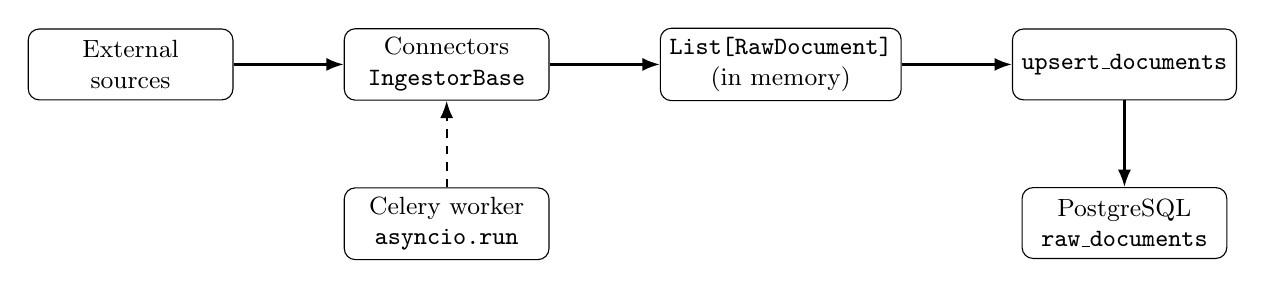
\begin{tikzpicture}[
  node distance=1.1cm and 1.4cm,
  box/.style={rectangle, draw, rounded corners, minimum width=2.6cm, minimum height=0.9cm, align=center, font=\small},
  arr/.style={-{Latex[length=2.2mm]}, thick},
]
  \node[box] (src) {External\\sources};
  \node[box, right=of src] (conn) {Connectors\\\texttt{IngestorBase}};
  \node[box, right=of conn] (raw) {\texttt{List[RawDocument]}\\(in memory)};
  \node[box, right=of raw] (store) {\texttt{upsert\_documents}};
  \node[box, below=of store] (db) {PostgreSQL\\\texttt{raw\_documents}};
  \node[box, below=of conn] (celery) {Celery worker\\\texttt{asyncio.run}};
  \draw[arr] (src) -- (conn);
  \draw[arr] (conn) -- (raw);
  \draw[arr] (raw) -- (store);
  \draw[arr] (store) -- (db);
  \draw[arr, dashed] (celery) -- (conn);
\end{tikzpicture}
\end{center}

Celery tasks (see \texttt{app/celery\_app.py}) instantiate a connector, run
\texttt{asyncio.run(connector.fetch())}, then pass the result list to
\texttt{upsert\_documents}.

\subsection{Module map}

\begin{description}
  \item[\texttt{app/ingestion/base.py}] Abstract base class \texttt{IngestorBase}.
  \item[\texttt{app/ingestion/web\_connector.py}] BFS web crawl (Scrapling), HTML extraction, optional LLM fallback, PDF/XML harvest.
  \item[\texttt{app/ingestion/pdf\_connector.py}] Download PDF, extract per-page text/tables (\texttt{pdfplumber}, optional Docling).
  \item[\texttt{app/ingestion/rss\_connector.py}] \texttt{feedparser}-based RSS/Atom/RDF $\rightarrow$ one document per entry.
  \item[\texttt{app/ingestion/xml\_connector.py}] \texttt{lxml} XPath for USLM / Akoma Ntoso / generic XML.
  \item[\texttt{app/ingestion/email\_connector.py}] IMAP + MIME; PDF attachments delegated to \texttt{PDFConnector}.
  \item[\texttt{app/ingestion/storage.py}] \texttt{upsert\_documents} (PostgreSQL \texttt{INSERT ... ON CONFLICT}).
  \item[\texttt{app/ingestion/url\_utils.py}] URL normalization, domain checks, spider-trap heuristics.
  \item[\texttt{app/ingestion/http\_utils.py}] TLS/\texttt{httpx} \texttt{verify} policy (truststore, CA bundles, optional host skip list).
  \item[\texttt{app/ingestion/artifact\_store.py}] Optional S3 uploads for raw HTML / extracted text.
  \item[\texttt{app/models.py}] \texttt{RawDocument} SQLModel table (among other domain models).
  \item[\texttt{app/config.py}] Pydantic settings (DB, Redis, OpenAI, IMAP, AWS, ingestion TLS flags).
\end{description}

%==============================================================================
\section{Canonical model: \texttt{RawDocument}}
%==============================================================================

Defined in \texttt{app/models.py}. Each ingested chunk (web page, RSS item, PDF page, XML section, email body) becomes one row.

\begin{itemize}
  \item \texttt{id}: UUID primary key.
  \item \texttt{source\_url}: provenance (entry link, page URL, PDF URL, etc.).
  \item \texttt{source\_type}: constrained to \texttt{web}, \texttt{pdf}, \texttt{rss}, \texttt{xml}, \texttt{email}.
  \item \texttt{raw\_text}, \texttt{title}, \texttt{language}: extracted content and optional ISO 639-1 language.
  \item \texttt{content\_hash}: SHA-256 hex digest of text; \textbf{unique} constraint \texttt{uq\_raw\_document\_content\_hash}.
  \item \texttt{fetched\_at}, \texttt{last\_seen\_at}: first capture and last re-ingest refresh.
\end{itemize}

The table \texttt{domains}, \texttt{urls}, \texttt{fetch\_runs}, \texttt{fetch\_attempts} models a richer crawl scheduler for future use; the current connectors primarily populate \texttt{raw\_documents}.

%==============================================================================
\section{\texttt{IngestorBase} contract}
%==============================================================================

\begin{lstlisting}
class IngestorBase(ABC):
    @abstractmethod
    async def fetch(self) -> List[RawDocument]: ...
\end{lstlisting}

Subclasses must return \textbf{unsaved} \texttt{RawDocument} instances with
\texttt{content\_hash} set consistently so \texttt{upsert\_documents} can deduplicate
without reading the database first.

%==============================================================================
\section{Connectors (detailed)}
%==============================================================================

\subsection{\texttt{WebConnector} (\texttt{web\_connector.py})}

\textbf{Role:} breadth-first crawl from \texttt{seed\_urls}, constrained by
\texttt{allowed\_domain}, optional \texttt{allowed\_path\_prefix}, \texttt{max\_pages},
\texttt{max\_depth}, and rate limiting (\texttt{rate\_limit\_rps}).

\textbf{Fetch pipeline:}
\begin{enumerate}
  \item \textbf{robots.txt}: \texttt{\_get\_robots} / \texttt{\_is\_allowed} via \texttt{httpx} (uses \texttt{httpx\_verify}).
  \item \textbf{Page fetch}: \texttt{\_fetch\_page} wraps Scrapling \texttt{StealthyFetcher} (fallback \texttt{DynamicFetcher}) in \texttt{run\_in\_executor} with \texttt{asyncio.wait\_for} hard cap (\texttt{PAGE\_TIMEOUT}).
  \item \textbf{HTTP status}: responses with status $\geq 400$ are skipped (no link expansion from that page).
  \item \textbf{Text extraction}: BeautifulSoup + boilerplate stripping + \texttt{markdownify}; short text triggers optional \texttt{\_llm\_extract} (OpenAI HTTP client verifies \texttt{api.openai.com} explicitly).
  \item \textbf{Deduplication}: normalized text hashed; duplicates skip adding another document to the in-memory list for the same crawl.
  \item \textbf{Link discovery}: \texttt{\_extract\_links}; PDF and XML links go to harvest sets; HTML links enqueue BFS if domain/path/trap checks pass.
  \item \textbf{Post-crawl harvest}: sequential \texttt{PDFConnector} / \texttt{XMLConnector} calls with \texttt{max\_pdfs} / \texttt{max\_xmls} caps and inter-request delay.
\end{enumerate}

\textbf{Important operational note:} persistence happens in the Celery task
\textit{after} the entire \texttt{fetch()} (HTML + PDF + XML) completes, not per page.

\begin{table}[h]
\centering
\begin{tabular}{@{}llp{7.2cm}@{}}
\toprule
Parameter & Typical & Meaning \\
\midrule
\texttt{seed\_urls} & list of URLs & BFS starting points (normalized, de-duplicated). \\
\texttt{allowed\_domain} & \texttt{www.example.gov} & Only enqueue same-site links (\texttt{is\_same\_domain}). \\
\texttt{allowed\_path\_prefix} & \texttt{/trade} or \texttt{/nota\_detalle} & Optional: only follow links whose path starts with this prefix. \\
\texttt{max\_pages} & 50 & Stop after this many HTML documents with extracted text. \\
\texttt{max\_depth} & 2--3 & Maximum BFS depth from seeds. \\
\texttt{rate\_limit\_rps} & 0.5--1.0 & Sleep between requests ($\approx 1/\mathrm{rps}$). \\
\texttt{max\_pdfs} / \texttt{max\_xmls} & 5--20 & Cap post-crawl PDF/XML connector invocations. \\
\texttt{harvest\_pdfs} / \texttt{harvest\_xml} & \texttt{True} & Collect links to PDF/XML during crawl. \\
\bottomrule
\end{tabular}
\caption{Main \texttt{WebConnector} constructor parameters (see source for defaults).}
\end{table}

\subsection{\texttt{PDFConnector} (\texttt{pdf\_connector.py})}

\textbf{Role:} download PDF from URL (or read local path), extract one logical chunk per page (table cells expanded to readable lines for testing requirements).

\textbf{Flow:} \texttt{\_get\_pdf\_bytes} (\texttt{httpx} with \texttt{httpx\_verify(source)}) $\rightarrow$ optional Docling $\rightarrow$ \texttt{pdfplumber} per page $\rightarrow$ skip very short pages $\rightarrow$ per-page \texttt{RawDocument} with \texttt{source\_type="pdf"}.

\subsection{\texttt{RSSConnector} (\texttt{rss\_connector.py})}

\textbf{Role:} \texttt{feedparser.parse(feed\_url)} (in thread pool), map each entry to a \texttt{RawDocument} with \texttt{source\_type="rss"}.

\textbf{Text assembly:} title, published time, summary, link concatenated into \texttt{raw\_text}; \texttt{source\_url} prefers entry link else feed URL; \texttt{content\_hash} over that text.

\subsection{\texttt{XMLConnector} (\texttt{xml\_connector.py})}

\textbf{Role:} download XML via \texttt{httpx} + \texttt{httpx\_verify(source)}, parse with \texttt{lxml}, detect USLM vs Akoma Ntoso vs generic, extract sections/articles, emit one \texttt{RawDocument} per substantial section.

\subsection{\texttt{EmailConnector} (\texttt{email\_connector.py})}

\textbf{Role:} IMAP connection using settings \texttt{IMAP\_*}; scan messages; build \texttt{RawDocument} bodies from plain/HTML parts; PDF attachments routed through \texttt{PDFConnector}.

%==============================================================================
\section{URL utilities (\texttt{url\_utils.py})}
%==============================================================================

\begin{itemize}
  \item \texttt{normalize\_url}: resolves relatives, strips tracking query params and fragments, lowercases scheme/host, stable query ordering.
  \item \texttt{is\_same\_domain}: allows subdomains and \texttt{www.} stripping vs \texttt{allowed\_domain}.
  \item \texttt{is\_spider\_trap}: long URLs, session id query params, calendar-like path segments, repeated path segments.
\end{itemize}

Used heavily by \texttt{WebConnector} when enqueueing links.

%==============================================================================
\section{HTTP/TLS helpers (\texttt{http\_utils.py})}
%==============================================================================

\texttt{httpx\_verify(url=None)} returns the \texttt{verify} argument for \texttt{httpx.AsyncClient}:
truststore-backed \texttt{SSLContext} when available, else explicit CA files
(\texttt{SSL\_CERT\_FILE}, Debian bundle, \texttt{certifi}).

Optional \texttt{INGEST\_TLS\_SKIP\_VERIFY\_HOST\_SUFFIXES} (comma-separated, from
\texttt{app/config.py}) disables verification for matching \textit{request} hosts only
(e.g.\ broken government certificate chains). OpenAI calls use verification tied to
\texttt{api.openai.com}, not the crawled page URL.

%==============================================================================
\section{Persistence (\texttt{storage.py})}
%==============================================================================

\texttt{upsert\_documents(documents)} opens a SQLModel session, and for each document executes PostgreSQL \texttt{INSERT ... ON CONFLICT (content\_hash) DO UPDATE SET last\_seen\_at = now()}.

Returns counts \texttt{inserted} vs \texttt{updated} (distinguished via
\texttt{inserted\_primary\_key} on the execution result).

Empty input returns zeros without touching the database.

\begin{lstlisting}[caption={Upsert pattern (conceptual; see \texttt{storage.py} for full SQLAlchemy API).}]
def upsert_documents(documents: List[RawDocument]) -> dict:
    if not documents:
        return {"inserted": 0, "updated": 0}
    with Session(engine) as session:
        for doc in documents:
            stmt = pg_insert(RawDocument).values(...).on_conflict_do_update(
                constraint="uq_raw_document_content_hash",
                set_={"last_seen_at": now},
            )
            session.execute(stmt)
        session.commit()
    return {"inserted": inserted, "updated": updated}
\end{lstlisting}

%==============================================================================
\section{Artifact store (\texttt{artifact\_store.py})}
%==============================================================================

If \texttt{AWS\_S3\_BUCKET} (and boto3) are configured, \texttt{upload\_artifacts} can store raw HTML and extracted text under a dated key prefix. If not configured, operations no-op. This is parallel to \texttt{raw\_documents} and can be wired from higher-level fetch flows.

%==============================================================================
\section{Celery orchestration (\texttt{celery\_app.py})}
%==============================================================================

\begin{itemize}
  \item \texttt{rss\_ingest\_task(feed\_url, ...)} $\rightarrow$ \texttt{RSSConnector} $\rightarrow$ \texttt{upsert\_documents}.
  \item \texttt{pdf\_ingest\_task(source, title)} $\rightarrow$ \texttt{PDFConnector}.
  \item \texttt{xml\_ingest\_task(source, title)} $\rightarrow$ \texttt{XMLConnector}.
  \item \texttt{email\_ingest\_task()} $\rightarrow$ \texttt{EmailConnector} (skips if IMAP not configured).
  \item \texttt{web\_crawl\_task(seed\_urls, allowed\_domain, max\_pages, max\_depth, rate\_limit\_rps, allowed\_path\_prefix, max\_pdfs, max\_xmls)} $\rightarrow$ \texttt{WebConnector}.
\end{itemize}

Beat schedule (excerpt): RSS feeds every 30 minutes; web crawls for EUR-Lex, FCA, Federal Register every 6 hours; heartbeat every 5 minutes.

Tasks use \texttt{asyncio.run} because Celery workers are synchronous at the task entrypoint.

\begin{table}[h]
\centering
\begin{tabular}{@{}lp{9cm}@{}}
\toprule
Celery task & Connector and notes \\
\midrule
\texttt{rss\_ingest\_task} & \texttt{RSSConnector}; kwargs from Beat include \texttt{feed\_url}. \\
\texttt{web\_crawl\_task} & \texttt{WebConnector}; passes crawl caps and optional path prefix. \\
\texttt{pdf\_ingest\_task} & Single-source \texttt{PDFConnector} (on-demand or scheduled). \\
\texttt{xml\_ingest\_task} & Single-source \texttt{XMLConnector}. \\
\texttt{email\_ingest\_task} & \texttt{EmailConnector}; no-op style skip if IMAP unset. \\
\bottomrule
\end{tabular}
\caption{Celery tasks wrapping connectors + \texttt{upsert\_documents}.}
\end{table}

%==============================================================================
\section{Configuration (\texttt{app/config.py})}
%==============================================================================

Relevant environment-driven settings include \texttt{DATABASE\_URL}, \texttt{REDIS\_URL},
\texttt{OPENAI\_API\_KEY} / \texttt{OPENAI\_MODEL} (LLM fallback in web extraction),
IMAP and AWS blocks, and \texttt{INGEST\_TLS\_SKIP\_VERIFY\_HOST\_SUFFIXES}.

Docker Compose sets \texttt{SSL\_CERT\_FILE} / \texttt{REQUESTS\_CA\_BUNDLE} in the
\texttt{Dockerfile} for system CA paths inside the image.

%==============================================================================
\section{Dependencies (ingestion-related)}
%==============================================================================

See \texttt{requirements.txt}: \texttt{httpx}, \texttt{certifi}, \texttt{truststore},
\texttt{scrapling}, \texttt{beautifulsoup4}, \texttt{markdownify}, \texttt{lxml},
\texttt{pdfplumber}, \texttt{feedparser}, \texttt{langdetect}, optional \texttt{boto3},
\texttt{sqlmodel}/\texttt{psycopg2-binary}, \texttt{celery}/\texttt{redis}.

%==============================================================================
\section{How to build this PDF}
%==============================================================================

From \texttt{regulation-prj-v1/docs/}:
\begin{verbatim}
pdflatex -interaction=nonstopmode ingestion_layer.tex
pdflatex -interaction=nonstopmode ingestion_layer.tex
\end{verbatim}
Run \texttt{pdflatex} twice for stable references and table of contents.
Requires a LaTeX distribution (TeX Live, MiKTeX, etc.) with \texttt{listings} and \texttt{tikz}.

%==============================================================================
\section{Summary}
%==============================================================================

The ingestion layer is a \textbf{plugin family} of async connectors producing
\texttt{RawDocument} lists, plus \textbf{shared utilities} for URLs and TLS,
\textbf{centralized upsert} into PostgreSQL, and \textbf{Celery} for scheduling and
retries. The heaviest and most configurable path is \texttt{WebConnector} (crawl
limits, PDF/XML caps, extraction and LLM fallback); RSS is the lightest path for
many regulatory publishers that expose feeds.

\end{document}
